
\chapter{Introduction}

% 학위논문 주제 설정의 배경, 관련 분야에서 기존의 연구,
% 본 논문의 취지, 실험 논문의 경우 연구에 대한 간략한 소개와
% 연구를 위해 설정한 가설 등을 소개한다.

\section{Sequence Databases}

Next generation sequencing (NGS) technologies have revolutionized the way we collect and analyze biological data. Thanks to NGS, the cost of sequencing has dropped drastically and continued to decrease with more new technologies developed. Accompanying this change is the explosive growth of the amount of sequencing data and the size of sequence databases. The Sequence Read Archive (SRA) is one of the most popular and widely used sequence databases that store both private and public sequence reads and provide access in various foramts including the commonly used \texttt{FASTQ} file format. Its size has grown exponentially since 2008 and currently reached more than 60 petabytes large. The growth in size of Sequence Read Archive is visualized in \ref{fig:sra_stat}.



\section{State-of-the-art Algorithms for Sequence Searches}

\subsection{DIAMOND}

\subsection{MMseqs2}

\subsection{BIGSI}

\section{Prototype of Petasearch Algorithm}

\section{Motivation and Contribution of the Thesis}

\pagebreak

\thispagestyle{empty}
\begin{figure}[t]
  \centering
  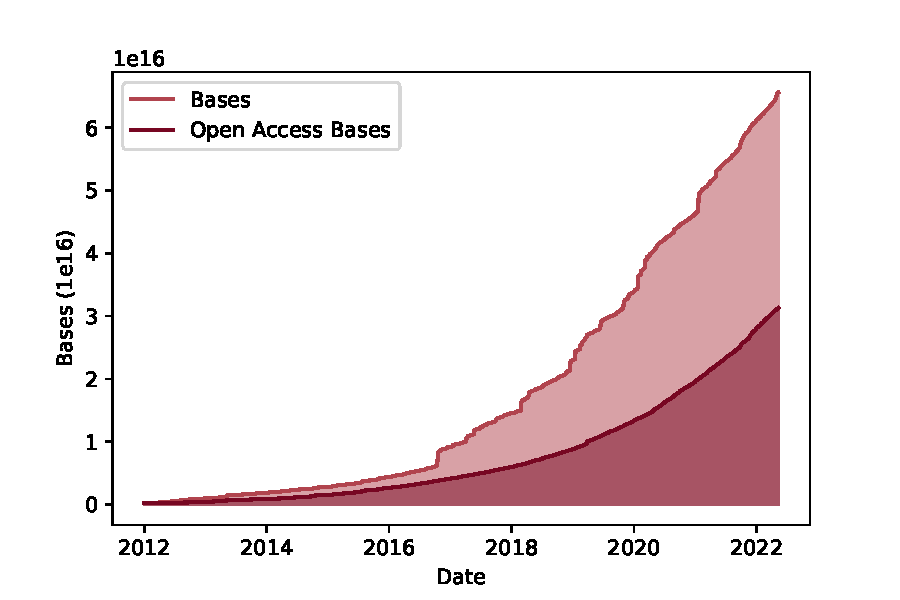
\includegraphics[width=\textwidth]{images/sra_stat.pdf}
  \caption{The exponential growth of the Sequence Read Archive from 2008 to 2022. The total amount of sequence data (unit in bases) and publicly available data are visualized in pink and dark red respectively.}
  \label{fig:sra_stat}
\end{figure}
